\chapter{Realization}

In the following chapter, we describe the realization of the software system. In section \ref{sec:structure}, we give an overview of the different components and how they interact with each other. In section \ref{sec:changes}, we list the changes which have to be made to existing components.

\section{Structure}\label{sec:structure}

The system consists of three major components: the \emph{Social Bot}, the \emph{Mensa Service} and the \emph{MobSOS} services. 

\subsection{MobSOS services}
The MobSOS services include the MobSOS Data Processing, MobSOS Success Modeling , MobSOS CCA GraphQl, MobSOS CCA REST services.

\subsubsection{MobSOS Data Processing}
The MobSOS Data Processing service collects logs from the Mensa service and the MobSOS Success Modeling service. Those logs contain informtion about how community members are using the service. The data is stored in the MobSOS MySQL database under the MESSAGE table. The table contains a column REMARKS which can be used to store arbitrary json data.

\subsubsection{MobSOS Success Modeling}
The MobSOS Success Modeling service is used to make the visualizations of success factors and measures defined by the community. The service stores success models per group and per service. 
The groups reflect the las2peer \emph{GroupAgent} and the services reflect the \emph{ServiceAgents} in the las2peer network.
The success model contains the six MobSOS dimensions:
\begin{itemize}
    \item System Quality
    \item Information Quality
    \item Use 
    \item User Satisfaction
    \item Individual Impact 
    \item Community Impact
\end{itemize}
Each of these dimensions includes a list of success factors.
Each factor contains a list of success measures. The success measures contain a \texttt{query} element which contains the SQL query and a \texttt{visualization} element which contains information about the visualization.

\subsubsection{MobSOS CCA GraphQL and REST}
The MobSOS CCA backend service has access to three different databases. First, the MobSOS CCA service can access the food reviews, which are stored inside the las2peer database of the Mensa Service. Second, the system can access \emph{Mediabase} data, which contains data from reviews, made outside of the las2peer system. 
% This data could be collected by a crawler bot, which searches Google and Twitter for reviews of the canteen. Those two databases provide the information quality factors of the MobSOS success model.
Third, the CCA service can also access monitoring data generated by the Bot and the Mensa Service. 
% Those monitoring messages provide the system quality factors of the MobSOS success model.

\subsection{Mensa Service}

\subsection{Bot Service}

The Bot Service acts as an interface between the user, and the las2peer backend services.
The Bot Service communicates with the \emph{Mensa Service} in order to get the menu for the canteen. Additionally, the bot can send requests to the Mensa service, telling it to add, or modify, reviews.

The Bot Service communicates with the MobSOS Success Modeling system in order to get visualisations of the success model. Furthermore, it can also be used to modify the success model of the community. 
The bot sends the resulting visualisations to the user in chat.
The bot is modeled with the help of the Social Bot Framework frontend canvas and deployd on the las2peer social bot manager service.



\section{Additional services}
Some additional systems were deployed or added during my work.

\subsection{Mensa Guide}
The Mensa Guide service is a frontend to the las2peer mensa service. It provides basic functionalities like the menu for mensas in Aachen, making reviews and uploading pictures for dishes.

\subsection{MobSOS evaluation center}
The MobSOS evaluation center is a service which communicates with the MobSOS backend services. It provides a range of functionalities. Those include: contact management and group management. 
It also allows community members to editing existing success models or create new ones.
Furthermore it also provides visualizations for the measures of the success model, which it gets from the MobSOS query visualization service.

\subsection{MobSOS query visualization service}
The MobSOS query visualization service is a las2peer service which can be used to make visualizations data in a database. It also allows users to add new database and store SQL queries.

\subsection{Data2chart}
This service was written by me\footnotemark in order to render google charts as an image which could be sent to the chatbot and visualized in the chat. This service was created as an alternative to the MobSOS query visualization service which did not provide the option to render the chart as an image. 
\footnotetext{\url{https://github.com/lakhoune/image-renderer}}
The service is written in NodeJs and uses an npm library called google-charts-node\footnotemark.
\footnotetext{\url{https://www.npmjs.com/package/google-charts-node}}

This module creates an html file which loads the google charts and then renders that html file in a headless browser \footnotemark and returns the resulting image.
\footnotetext{\url{https://www.npmjs.com/package/puppeteer}}
The MobSOS success modeling service calls this service if a bot is requesting a visualization. It includes the data for the graph in a post request which has the following form:

\begin{lstlisting}
POST  http://localhost:3000/ HTTP/1.1
content-type: application/json

{
    "data": [...],
    "chartType":"BarChart",
    "options":{
        "title":"Chart title",
        "hAxis":{
            "title":"Axis title"
        }
    },
    "clean":true 
}
\end{lstlisting}


\section{Changes to Core Components} \label{sec:changes}
\begin{figure}[h]
    \centering
    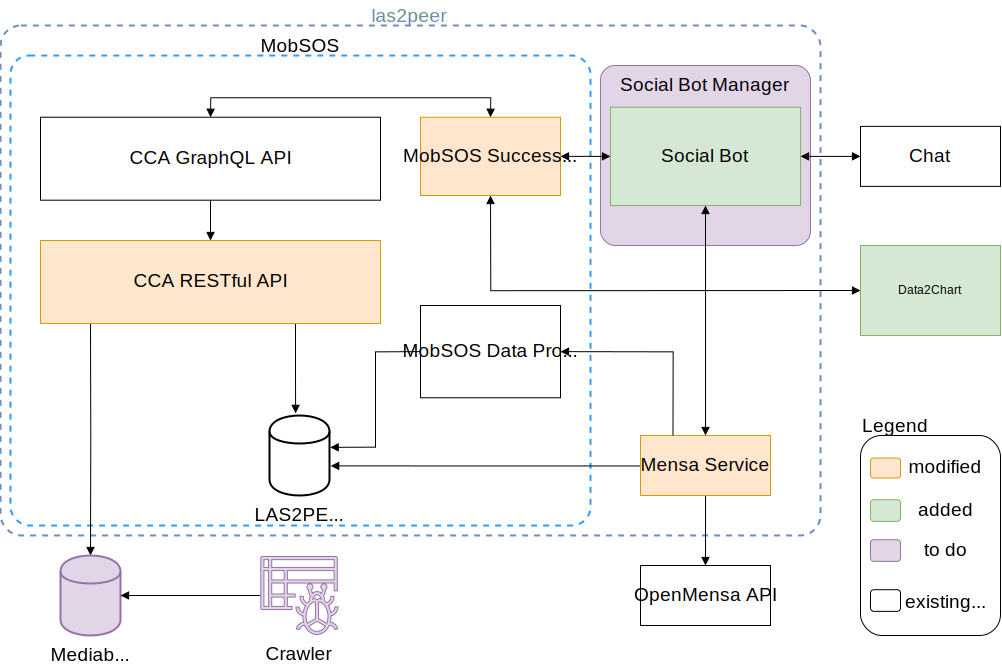
\includegraphics[width=\linewidth]{realization/components_overview.png}
    \caption{Overview of the different components}
    \label{fig:componentsOverview}
\end{figure}
\subsection{MobSOS Success Modeling}
The measure definition was extended with a \texttt{database} element which is part of the query and which gives additional information about which database the query should be executed on. The attributes for the \texttt{database} element are \texttt{name} and \texttt{dbSchema}. The name identifies the database on the graphql server. The \texttt{dbSchema} describes which schema should be used.
Both of these attributes can be omitted. In this case, when the graphql query is prepared the default database and default database schema are used, which are \texttt{las2peer} and \texttt{LAS2PEERMON} respectively.
This allows the community to visualize data from any database supported by the graphql service.

\subsection{Social Bot Framework}
The Social Bot Framework needs to be extended, such that the bot is able to listen to specific mentions in group chats and filtering out the rest of the conversations, such that the bot can be integrated in group chats, as a quiet agent.

A metion has the following form \texttt{@botname}, where \emph{botname} represents the username that the bot has in the Slack channel.

\subsubsection{Social Bot}
The Social Bot will be created, using the SBF frontend service.
The first feature, which will be implemented is quering the menu for a specific canteen. Next the review process will be implemented as a question-based dialogue. An example can be seen in figure \ref{fig:chatMockup}.
Both of these features should be implemented as soon as possible, to allow the collection of food review and such that the first phase of the evaluation can be done (see Chapter \ref{cha:eval}).
The food reviews will be done in private chat with the bot. The menu query should be available both in private chat and in channels, given that the SBF is already extended to allow for mentions.

The next feature, which will be implemented is the visualisation of success variables. Users should be able to formulate GraphQL queueries, which will be recognized by the bot to run the visualisations. Additionally, templates will be available, which are to be run when specific intents are recognized, such that the query visualisations can be done in an intuitive way. An example can be seen in figure \ref{fig:visualReq}.

Finally the success modeling will be implemented. Users should be able
to modify the success model in chat. Therefore, an update routine needs to be implemented, which is started at the recognition of a specific intent.

\subsection{MobSOS CCA}
The MobSOS CCA system needs to be extended such that the success model data can be visualized and sent as a picture to the user. Therefore, the Google Charts API will be used in combination with an HTML renderer, which will render the visualizations which were produced by the Charts API and send them back as a PNG to the Bot Service.

\subsection{Google Charts API}
Google Charts API\footnotemark is an API that provides visualizations for database data. The data, which should be visulaized needs to be wrapped inside a Javascript class called \texttt{DataTable}, which represents a two-dimensional table with rows and columns, where each column has a datatype.
A new column can be added using the \texttt{DataTable.addColumn} function, which takes the type and name as input. An example can be seen in Listing \ref{lst:gglCharts} from the Google Charts API documentation\footnotemark[\value{footnote}].

\begin{lstlisting}[caption=Example use of the DataTable class,captionpos=b,label={lst:gglCharts}]
var data = new google.visualization.DataTable();
data.addColumn('string', 'Topping');
data.addColumn('number', 'Slices');
data.addRows([
	['Mushrooms', 3],
	['Onions', 1],
	['Olives', 1], 
	['Zucchini', 1],
	['Pepperoni', 2]
]);
\end{lstlisting}

The visualizations are rendered as SVGs in the browser, but can be the PNG file can be accessed by maken an http call with the \texttt{getImageURI} as image URI parameter.

\footnotetext{\href{https://developers.google.com/chart}{Google Charts API}}


\begin{figure}
    \centering
    \includegraphics[height=0.45\textheight]{realization/chat_mockup.png}
    \caption{Example use of community Service with the Bot}
    \label{fig:chatMockup}
\end{figure}

\begin{figure}
    \centering
    \includegraphics[height=0.45\textheight]{realization/visual_req.png}
    \caption{Example of a chat interaction with the Bot}
    \label{fig:visualReq}
\end{figure}